% Solution of the problem with Russian in tikzposter: https://tex.stackexchange.com/questions/307054/use-cyrillic-characters-in-tikzposter

% we don't want ae.sty
\expandafter\def\csname ver@ae.sty\endcsname{}

\documentclass[20pt, a3paper, portrait,
blockverticalspace=10mm]{tikzposter}

% Adding logos
\makeatletter
\newcommand\insertlogoi[2][]{\def\@insertlogoi{\includegraphics[#1]{#2}}}
\newcommand\insertlogoii[2][]{\def\@insertlogoii{\includegraphics[#1]{#2}}}
\newlength\LogoSep
\setlength\LogoSep{0pt}

\insertlogoi[width=7cm]{MEPhI_logo}
\insertlogoii[width=7cm]{Julich_logo}

\renewcommand\maketitle[1][]{  % #1 keys
	\normalsize
	\setkeys{title}{#1}
	% Title dummy to get title height
	\node[transparent,inner sep=\TP@titleinnersep, line width=\TP@titlelinewidth, anchor=north, minimum width=\TP@visibletextwidth-2\TP@titleinnersep]
	(TP@title) at ($(0, 0.5\textheight-\TP@titletotopverticalspace)$) {\parbox{\TP@titlewidth-2\TP@titleinnersep}{\TP@maketitle}};
	\draw let \p1 = ($(TP@title.north)-(TP@title.south)$) in node {
		\setlength{\TP@titleheight}{\y1}
		\setlength{\titleheight}{\y1}
		\global\TP@titleheight=\TP@titleheight
		\global\titleheight=\titleheight
	};
	
	% Compute title position
	\setlength{\titleposleft}{-0.5\titlewidth}
	\setlength{\titleposright}{\titleposleft+\titlewidth}
	\setlength{\titlepostop}{0.5\textheight-\TP@titletotopverticalspace}
	\setlength{\titleposbottom}{\titlepostop-\titleheight}
	
	% Title style (background)
	\TP@titlestyle
	
	% Title node
	\node[inner sep=\TP@titleinnersep, line width=\TP@titlelinewidth, anchor=north, minimum width=\TP@visibletextwidth-2\TP@titleinnersep]
	at (0,0.5\textheight-\TP@titletotopverticalspace)
	(title)
	{\parbox{\TP@titlewidth-2\TP@titleinnersep}{\TP@maketitle}};
	
	\node[inner sep=0pt,anchor=west] 
	at ([xshift=-\LogoSep]title.west)
	{\@insertlogoi};
	
	\node[inner sep=0pt,anchor=east] 
	at ([xshift=\LogoSep]title.east)
	{\@insertlogoii};
	
	% Settings for blocks
	\normalsize
	\setlength{\TP@blocktop}{\titleposbottom-\TP@titletoblockverticalspace}
}
\makeatother

% language settings
\usepackage[T2A]{fontenc}
\usepackage[utf8]{inputenc}
\usepackage[russian]{babel}

% scaling russian letters
\makeatletter
\newcommand{\xEC@family}[5]{%
	\DeclareFontShape{#1}{#2}{#3}{#4}%
	{<-5.5>#50500
		<5.5-6.5>#50600
		<6.5-7.5>#50700
		<7.5-8.5>#50800
		<8.5-9.5>#50900
		<9.5-10.5>#51000
		<10.5-11.5>#51095
		<11.5-13>#51200
		<13-16>#51440
		<16-18>#51728
		<18-21>#52074
		<21-26.88>#52488
		<26-32>#52986
		<32->#53583}{}}
\DeclareFontFamily{T2A}{cmr}{}
\xEC@family{T2A}{cmr}{m}{n}{larm}
\xEC@family{T2A}{cmr}{m}{sl}{lasl}
\xEC@family{T2A}{cmr}{m}{it}{lati}
\xEC@family{T2A}{cmr}{m}{sc}{lacc}
\xEC@family{T2A}{cmr}{bx}{n}{labx}
\xEC@family{T2A}{cmr}{b}{n}{larb}
\xEC@family{T2A}{cmr}{bx}{it}{labi}
\xEC@family{T2A}{cmr}{bx}{sl}{labl}
\xEC@family{T2A}{cmr}{bx}{sc}{laxc}
\xEC@family{T2A}{cmr}{m}{ui}{laui}
\makeatother

% or wrapping long titles
\makeatletter
\def\title#1{\gdef\@title{\scalebox{\TP@titletextscale}{%
			\begin{minipage}[t]{\linewidth}
				\centering
				#1
				\par
				\vspace{0.5em}
			\end{minipage}%
}}}
\makeatother

\title{Моделирование спин-орбитальной динамики пучка в накопительном кольце}
\author{Александр Аксентьев}
\date{\today}
\institute{НИЯУ ``МИФИ,'' Forschungszentrun J\"ulich}

\usepackage{blindtext}
\usepackage{comment}
\usepackage{url}

\usetheme{Basic}
\usecolorstyle{Russia}
\usebackgroundstyle{Empty}
\useblockstyle{Minimal}
\usetitlestyle{Default}
\colorlet{blocktitlefgcolor}{black}
\colorlet{titlefgcolor}{white}
%\colorlet{titlebgcolor}{blue!50!black!50}


\begin{document}
	\maketitle
	\block{Две концепции накопительного кольца}{
		Для проведения эксперимента по измерению Электрического Дипольного Момента (ЭДМ) дейтрона существует две парралельных концепции: кольцо с Замороженным Спином (Frozen Spin), и кольцо с Квази-замороженным Спином (QFS). В FS структуре спин частиц сонаправлен с её импульсом в любой момент времени; для этого требуется выполнение условия замороженности спина: равенство энергии частицы её т.н.``магической энергии.'' FS кольцо позволяет максимизировать полезный сигнал, однако практически невозможно обеспечить выполнение FS условия для ансамбля частиц. QFS структура ослабляет требование \emph{непрерывной} сонаправленности спина и импульса, требуя лишь усреднённой сонаправленности за один оборот. Цена за это упрощение --- некотороая деградация полезного сигнала (на уровне нескольких процентов). Задача настоящей работы --- исследовать какая из структур предпочтительнее для достижения необходимой точности измерения дЭДМ. Для этого необходимо смоделировать спин-орбитальную динамику пучка в обоих кольцах.
	}

%	\block{Численное моделирование динамики пучка}{
%		Существует два подхода к решению систем ОДУ: классическое пошаговое интегрирование (схемы Рунге-Кутты), и построение отображения начального состояния системы в конечное.
%	}
%	\begin{columns}
%		\column{.5}
%		\block{Пошаговое интегрирование}{
%			Система ОДУ решается для каждого начального условия, в каждый момент времени, в связи с чем такие методы мало-производительны при моделировании динамики большого ансамбля частиц на большом количестве оборотов в ускорителе. На данный момент, в разрабатываемом приложении имплементирована только пошаговая схема.
%			\begin{tikzfigure}
%				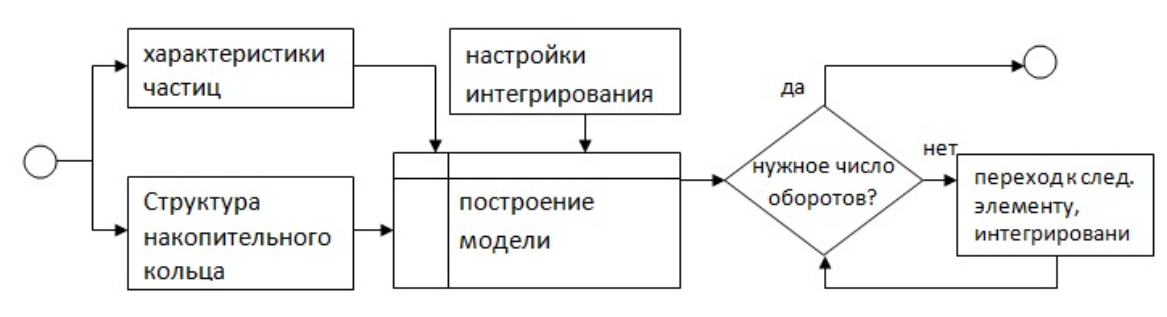
\includegraphics[width=.4\textwidth]{ODE_solution_RK}
%			\end{tikzfigure}
%		}
%		\column{.5}
%		\block{Матричное отображение}{
%			Пошаговое интегрирование производится только для одного оборота, результирующее отображение не зависит от начальных условий. Таким образом, построив отображение кольца, можно его использовать многократно, для разных начальных условий. 
%			\begin{tikzfigure}
%				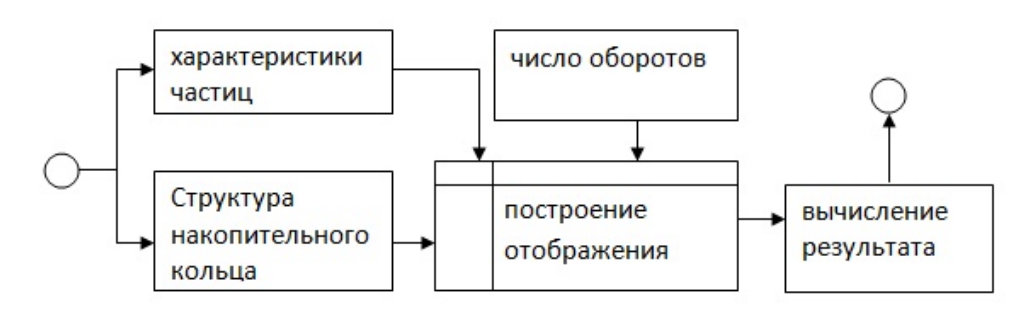
\includegraphics[width=.4\textwidth]{ODE_solution_Map}
%			\end{tikzfigure}
%		}
%	\end{columns}

	\begin{columns}
		\column{.5}
		\block{Описание работы приложения}{
			Программа пишется на языке Python с использованием пакетов numpy (контейнеры данных) и scipy (имплементация интегратора ОДУ). Отдельно, посредством класса \textbf{Particle} задаются параметры (масса, кинетическая энергия, магнитная аномалия) референсной частицы; ансамбль начальных условий (\textbf{StateList}); элементы кольца (\textbf{MQuad}, \textbf{MDipole}), и его структура (класс \textbf{Lattice}). Элементы структуры задают электромагнитные поля, использующиеся в правой части (\textbf{RHS}) системы ОДУ. 
			
			Вычисления проводятся в локальнаой системе координат $(\hat x, \hat y, \hat s)$, т.е., координаты референсной частицы на протяжении всей траектории равны 0. Моделирование погрешности установки элемента производится посредством вызова метода tilt\_($...$) базового класса \textbf{Element}, которая вычисляет матрицу наклона системы координат в месте установки элемента. Результат вычисления поля для данного вектора состояния системы затем умножается на эту матрицу.
			
			Для одновременного интегрирования ОДУ по всему ансамблю начальных условий, правая часть векторизована.
			
			Вычисление фазовых траекторий делегировано объекту класса \textbf{Tracker}, который инициализирует \textbf{RHS} объект, содержащий правую часть системы ОДУ, на основе данных об используемых структуре, частице, и ансамбле начальных условий.
			
		}
	
		\block{Текущие проблемы}{
			Среди известных на данный момент проблем, в порядке убывания срочности разрешения:
			\begin{itemize}
				\item При моделировании QFS структуры было обнаружено, что спин частиц свободно прецессирует. Проверка результатов с помощью аналитического выражения для частоты прецессии спина (уравнение Т-БМТ) выявила, если данный автор всё вычисляет правильно, различие аналитической и трекинговой частоты прецессии для элементов кроме диполя. Причины пока не известны.
				\item Из-за необходимости использования циклов по элементам структуры и по оборотам, интерпретируемый код очень медленный. Для решения этой проблемы планируется переписать некоторые (закрытые для пользователя) части кода на языке Cython.
			\end{itemize}
		}
		\column{.5}
		\block{Основные классы}{
			\begin{itemize}
				\item \textbf{Particle} содержит данные о физических параметрах референсной частицы (масса, энергия), а также методы их вычисления (импульс, Лоренц-фактор).
				\item \textbf{Element} родительский класс, из которого наследуются \textbf{MQuad} (магнитный квадруполь), \textbf{MSext} (магнитный секступоль), \textbf{MDipole} (магнитный диполь), \textbf{Wien} (Вин-фильтр), и т.д. Элементы содержат функции электромагнитных полей, и могут быть наклонены в 3D для симуляции погрешности установки элемента. 
				\item \textbf{Lattice} содержит в себе последовательность элементов структуры. Несколько Lattice-объектов (сегментов) можно собрать в один; эта функция была вызвана необходимостью вывода траекторий частиц внутри отдельных сегментов полной структуры.
				\item \textbf{PLog} хранит и рисует проинтегрированные траектории; также записывает данные на диск в формате hdf5.
				\item \textbf{RHS} инициализирует и вычисляет векторизованную правую часть системы ОДУ для заданного ансамбля.
				\item \textbf{Tracker} административный объект для ``прогонки'' начальных условий через Lattice-объект. Результат работы --- объект класса \textbf{PLog}.
			\end{itemize}
		}
		\block{Сравнение аналитики и трекинга}{
			Ниже представлены примеры расхождения значений, и производной по $s$, компоненты спина $S_x$, вычисленных по аналитическим формулам 
			\[
			\frac{d\vec S}{ds} = \frac{d\vec S}{dt} \cdot \frac{dt}{ds} = \underbrace{(\vec\Omega\times\vec{S})}_{T-BMT}\cdot t',
			\]
			\[
			S_x(t) = sin(\Omega\cdot t),
			\]
			и вычисленным в результате трекинга, для различных начальных условий.
		}
	\end{columns}
		
	\block{}{
		\begin{center}
			\begin{minipage}{.48\linewidth}
				\begin{tikzfigure}[Диполь]
					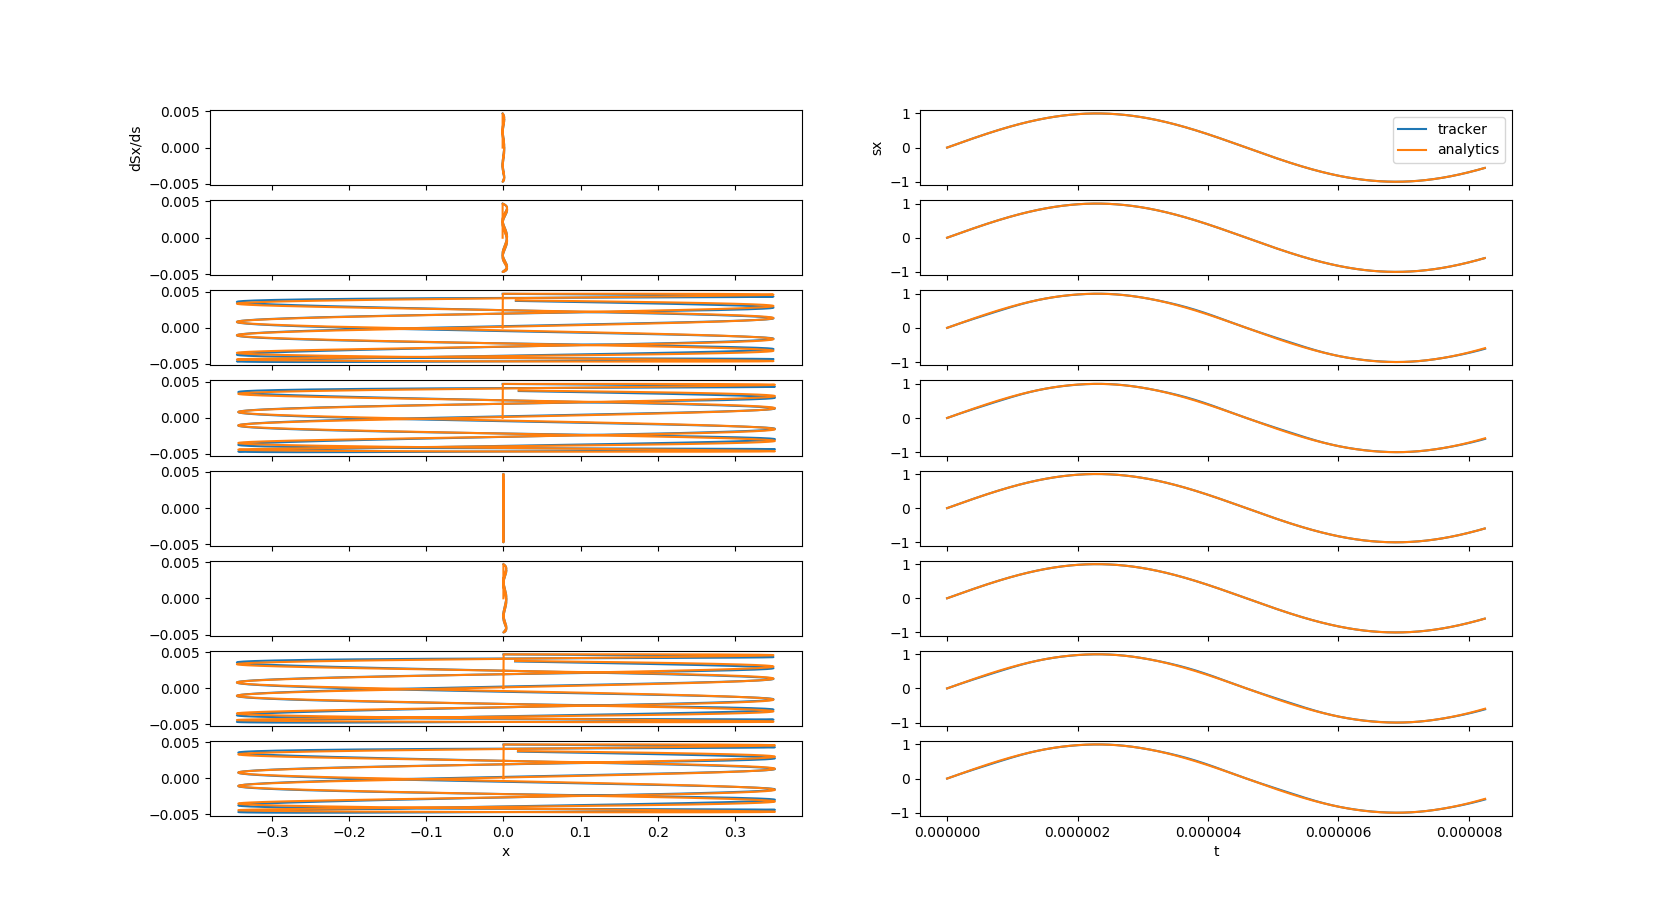
\includegraphics[scale=.95]{Dipole_test}
				\end{tikzfigure}		
			\end{minipage}
		\begin{minipage}{.48\linewidth}
			\begin{tikzfigure}[Вин-фильтр]
				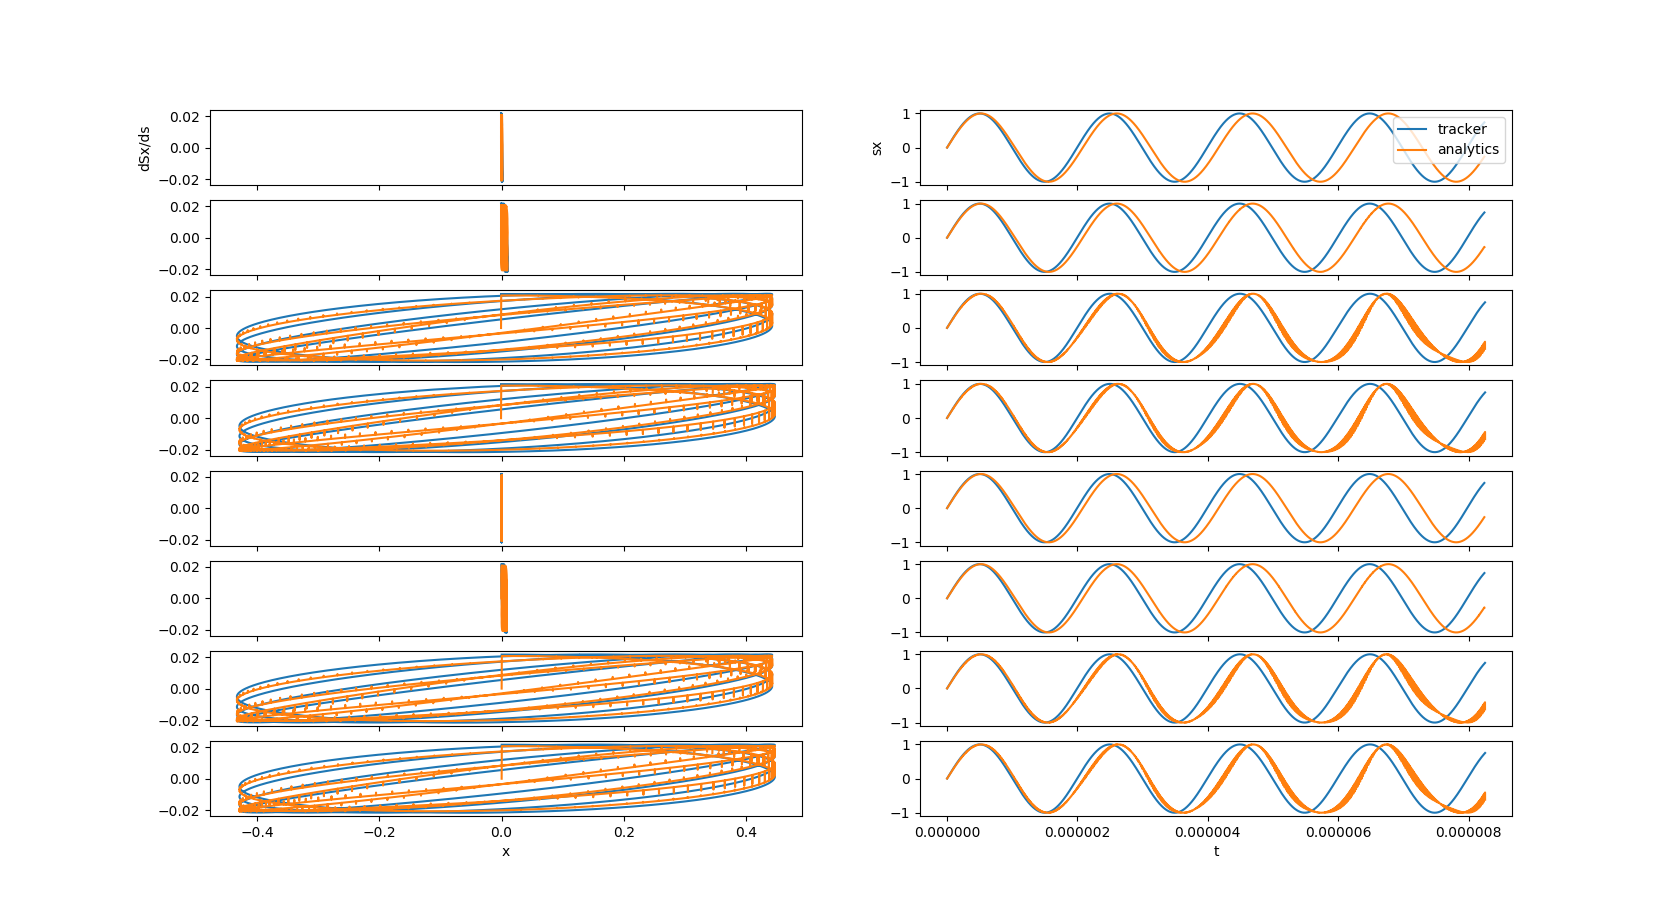
\includegraphics[scale=.95]{Wien_test}
			\end{tikzfigure}
		\end{minipage}
		\begin{tikzfigure}[Квадруполь]
			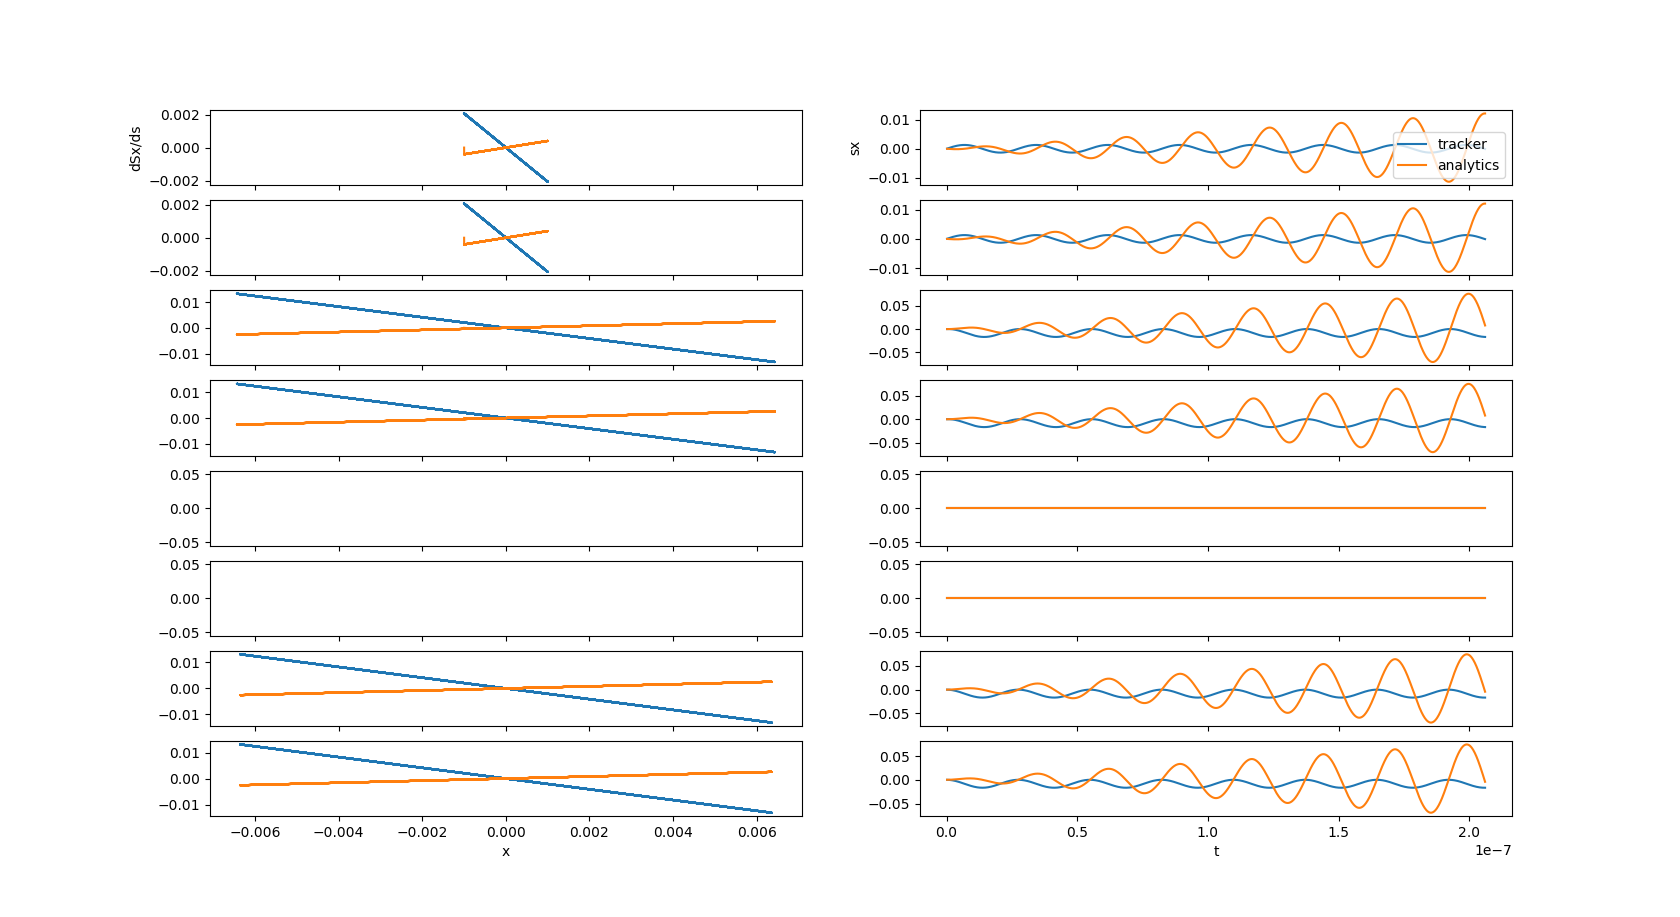
\includegraphics[scale=.95]{Quad_test}
		\end{tikzfigure}
		\end{center}
	}
\end{document}